\chapter{تعریف مسئله و مفاهیم مقدماتی}
\section{مروری بر موسیقی}
بدون شک موسیقی یکی از غنی‌ترین و قدیمی‌ترین بخش‌های تمدن بشری هست. اولین ساز
حدود چهل و پنج هزار سال پیش ساخته شد و تا امروز این شکل هنر به رشد خود ادامه‌
داده است. در این بخش مروری کوتاه بر مفاهیم موسیقیایی استفاده شده در این
پایان‌نامه انجام شده است.

\subsection{نت موسیقی}
مهم‌ترین بخش پایه‌ای موسیقی نت هست که می‌توان آن را با سه مفهوم \gls{pitch}،
\gls{velocity} و \gls{timber} توصیف کرد. \gls{pitch} فرکانس پایه‌‌ی صوت تولید
شده توسط ساز هست. \gls{pitch} واضح‌ترین فرکانس قابل درک نت هست. \gls{pitch}
زیرتر به معنی فرکانس بالاتر هست. \gls{velocity}، قدرت نواختن نت را مشخص می‌کند.
نت‌های که \gls{velocity} بالاتری دارند قابل درک‌تر هستند. همچنین معمولا نت اول
هر کلمه موسیقیایی \gls{velocity} بالاتری دارد. درنهایت \gls{timber} اشاره به شکل
سیگنال صوت تولید شده دارد. دو نت می‌توانند \gls{pitch} یکسانی داشته باشند ولی
شکلی که این نوسان انجام می‌شود متفاوت باشد. این تفاوت را با \gls{timber} ساز
بیان می‌کنند. \gls{timber} مفهومی هست که باعث تفاوت صدای سازهای مختلف می‌شود. در
شکل۱.۱ نمونه‌ای از \gls{timber} ساز ویولن نشان داده شده است.
\begin{figure}
    \centering
    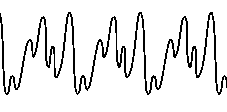
\includegraphics[height=2.5cm]{./statics/note_visualized.png}
    \caption{نمونه‌ای از \gls{timber} ویولن}
\end{figure}

همچنین هر نت یک زمان شروع یا onset و یک زمان پایان یا offset دارد. هرچند در بعضی
از سازها این مرزها کاملا مشخص و قابل تفکیک نمی‌باشند. برای مثال در پیانو پس از
رها کردن یک کلاویه همچنان ساز می‌تواند صوتی تولید کند.

وقتی از نواختن چند نت به صورت همزمان صحبت می‌کنیم معمولا مجموعه‌ای از نت‌ها با
هم صدایی خوش‌آیندتر تولید می‌کنند. به این مجموعه‌ی نت یک \gls{chord} گفته
می‌شود. یک \gls{chord} معمولا شامل نت‌هایی می‌شود که هارمونیک مشابه و نزدیک به
هم دارند. نت‌هایی که فرکانس پایه‌های آن‌ها با هم نسبت ۴، ۵، ۶ دارند نمونه‌ای از
یک \gls{chord} معروف هستند. به عنوان نمونه‌ای دیگر از \glspl{chord} مشهور
می‌توان به دو نت با نسب فرکانسی ۱ و ۲ اشاره کرد.

\subsection{پیانو}
پیانو یک ساز از خانواده ساز‌های صفحه‌کلیددار است که در سال ۱۶۹۸ اختراع شد. این
ساز در حالت استاندارد شامل ۸۸ کلید یا به اصلاح کلاویه هست که هرکدام نماینده یک
نت هستند. یکی از خصوصیات جالب این ساز این هست که پس از این که نوازنده شروع به
نواختن یک نت کرد تنها کنترلی که بر روی آن می‌تواند اعمال کنند یا رها کردن کلاویه
هست که باعث افت در شدت صدا می‌شود و یا دوباره نواخت همان نت هست.

همچنین این ساز شامل چندین پدال هست. مهمترین این پدال‌ها، پدال \gls{sustain} هست
که در صورتی که توسط نوازنده فشرده شده باشد، حتی رها کردن کلاویه باعث می‌شود صدای
آن نت باقی بماند. درنتیجه حتی اگه کلاویه متناظر یک نت هم فشرده نباشد باز آن نت
فعال می‌ماند.

\subsection{نمایش موسیقی}
همانند زبان طبیعی، برای موسیقی هم راه حلی نیاز هست که بتوان آن را ذخیره و به
سایرین منتقل کرد. همانند زبان طبیعی، نمایش‌های مختلفی نیز برای موسیقی وجود دارند
که بعضی‌ از آن‌ها مختص یک ساز خاص هستند. در ادامه سعی می‌شود چندتا از نمایش‌های
استفاده شده در این پایان‌نامه بررسی شوند.

\subsubsection{\gls{sound wav}}
از دید فیزیکی موسیقی چیزی بجز تغییر در فشار هوا و نوسان ذرات ماده نیست. با کمک
پیشرفت تکنولوژی می‌تواند از نوسانات را طی اجرای یک قطعه موسیقی در طول زمان
اندازه گرفت و با ایجاد مجدد نوسانات مشابه موسیقی را باز تولید کرد.

از این نمایش بیشتر در بحث‌های پردازش سیگنال مورد توجه قرار می‌گرد. برای استفاده
از این نمایش در کامپیوتر ابتدا نیاز هست تا این نمایش گسسته‌سازی شود.

\subsubsection{\gls{midi}}
در یک فایل \gls{MIDI} شروع، پایان، شدت، نواک و بسیاری دیگر از اطلاعات مربوط به
یک نت را می‌توان ذخیره کرد. همچنین این نمایش راه‌کارهایی برای تغییرات پدال‌ها و
سایر اطاعات اضافه نیز دارا می‌باشد. در نتیجه یک فایل \gls{MIDI} تمام اطاعات لازم
برای باز اجرای کامل یک قطعه موسیقی را دارا می‌باشد. با این حال این نمایش خوانایی
کمی‌ دارد و ساختار کلی موسیقی را رعایت نمی‌کند. برای همین استفاده از این نمایش
محدود به ارتباط بین ابزارهای دیجیتال هست.

\subsubsection{\gls{pianoroll}}
\gls{pianoroll} نمایشی دیگری هست که به صورت سنتی برای اجرای موسیقی به صورت
خودکار استفاده می‌شده است. این نمایش یک رول بزرگ هست که هر سطح این رول نماینده
یک زمان و هر ستون آن نماینده یک نت هست. خانه‌هایی که نت در آن‌ها فعال بود سوراخ
می‌شد تا ماشین بتواند آن را اجرا کند. با پیشرفت تکنولوژی این نمایش هم پیشرفت کرد
و بسیاری از نرم‌افزارهای مدرن از آن برای نمایش موسیقی استفاده می‌کنند.

به صورت کلاسیک این نمایش راهی برای نگه‌داری \gls{velocity} هر نت ندارند. برای
همین امروزه این اطلاعات به صورت جداگانه نگه‌داری می‌شوند. همچنین اطلاعاتی مثل
پلادها نیز در این نمایش جایی ندارند.
\begin{figure}
    \centering
    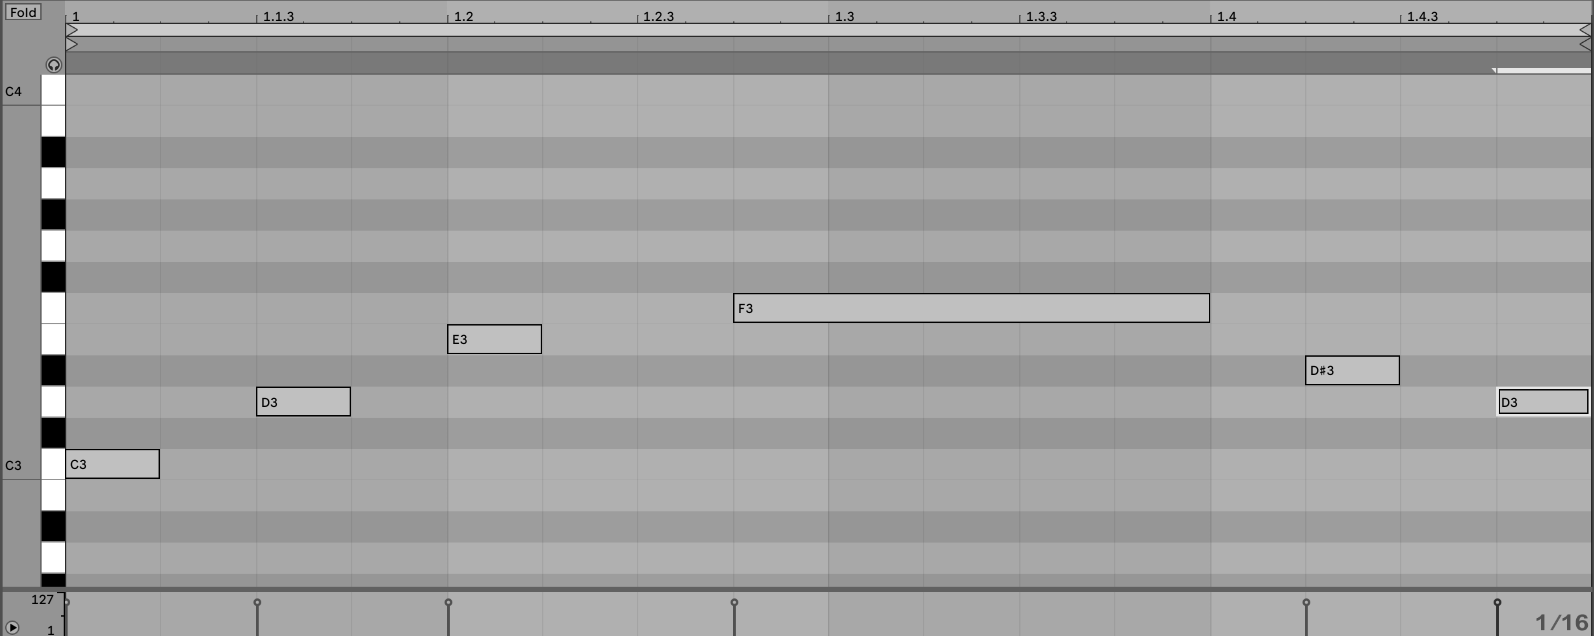
\includegraphics[width=12cm]{./statics/midi_piano_roll.png}
    \caption{نمونه‌ای از یک \gls{pianoroll} در یک نرم‌افزار کامپیوتری}
\end{figure}

\subsubsection{\gls{sheet music}}
این نمایش نمایشی هست که در مدارس موسیقی آموزش داده می‌شود و عمدتا به عنوان شکل
نوشتار استاندارد موسیقی شناخته می‌شود. بررسی کامل این نمایش خارج از دامنه‌ این
پایان‌نامه هست و به صورت مستقیم در این پایان‌نامه استفاده نمی‌شود. به صورت خلاصه
در این شکل از نمایش مجموعه \glspl{pitch}‌ مجاز و \glspl{duration}‌ مجاز مشخص
می‌شوند. سپس هر نت با توجه به مقدارهای تعریف شده بر روی خط‌های حامل نمایش داده
می‌شود.
\begin{figure}
    \centering
    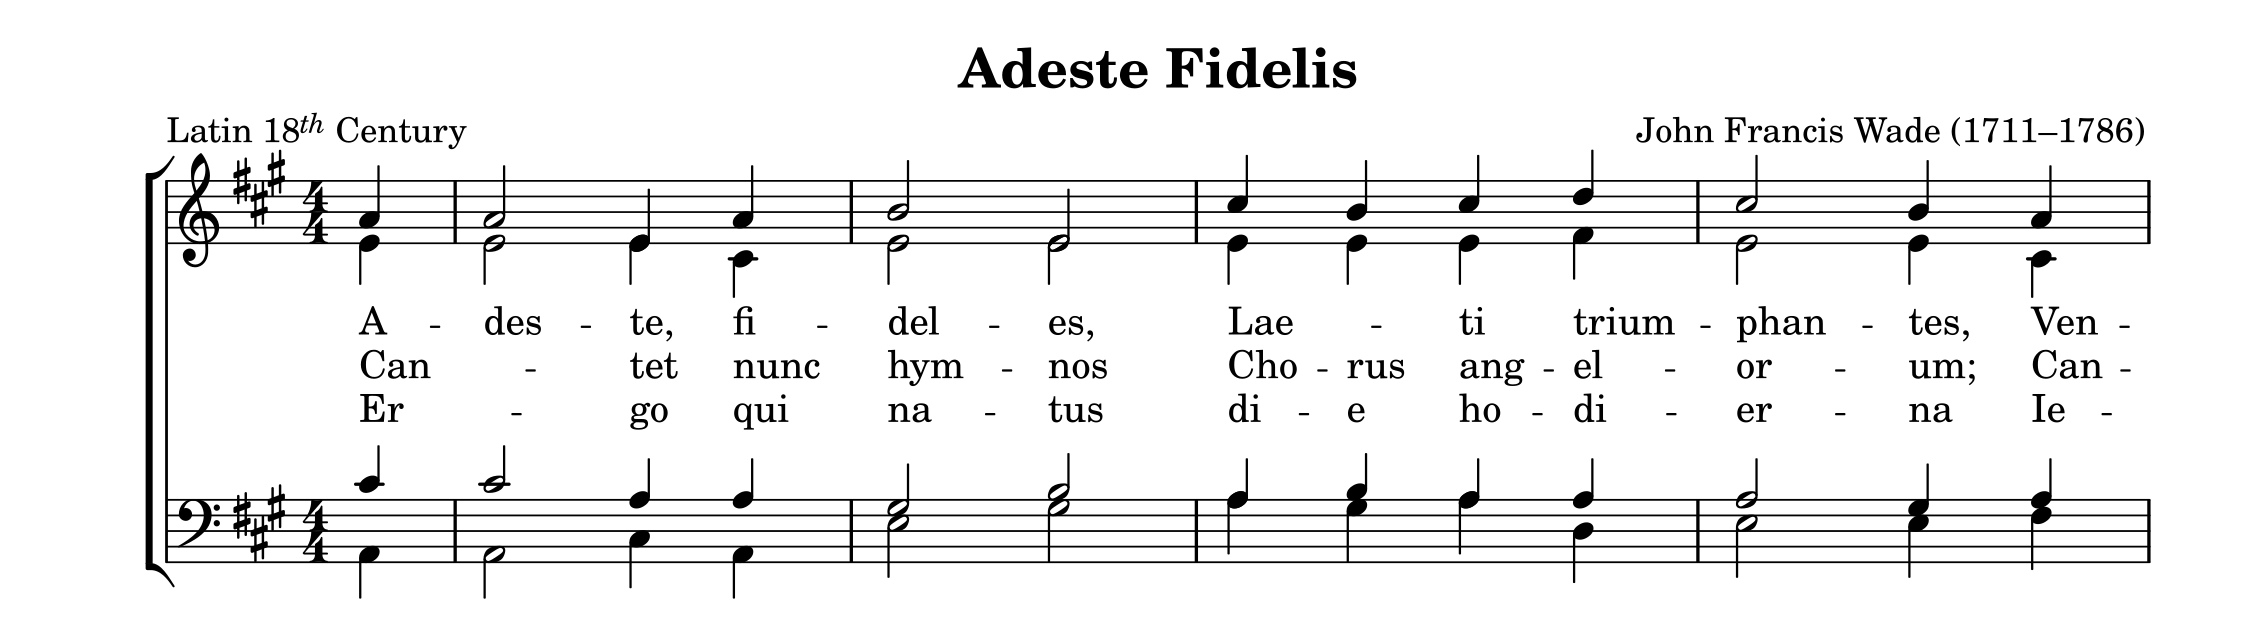
\includegraphics[width=12cm]{./statics/sheet_music.png}
    \caption{نمونه‌ای از یک \gls{sheet music}}
\end{figure}
